\chapter{EXPLOITING GPU}\label{exploitinggpu}
\section{Background}
\texttt{do} and \texttt{pardo} looping constructs are one of the most important
constructs in SIAL since they allow SIAL programmers to express operations on
blocks. Using \texttt{pardo} construct the calculations can be done in parallel.
SIAL runtime is responsible for the distribution of work over all the worker nodes.
In this chapter we present the problems faced in using GPU to execute the looping
constructs and how they were solved.

\subsection{Attempts in ACESIII}
There have been attempts\cite{Jindal2016} made in previous version of ACES
to use GPU to speed up computation. In this work the SIAL programmer had to deal
with a lot of low level GPU memory operations such as allocating memory on GPU,
copying blocks to and from GPU and deallocating memory on GPU. Since not all
calculations are suitable to be executed on GPU, the SIAL programmer had to mark
regions of SIAL code suitable to be executed on GPU.

\begin{lstlisting}[caption={Code Fragment from ACESIII for CCSD calculation},
  label={lst:ACESIII_gpucode}]
#start of GPU region
gpu_begin
#allocate and initialize blocks on GPU
gpu_put aoint(lambda,mu,sigma,nu) #allocate and copy data from CPU
DO i1
DO j1
    gpu_put LT2AOab1(mu,i1,nu,j1)
    gpu_put LT2AOab2(nu,j1,mu,i1)
    gpu_put LTAOab(lambda,i1,sigma,j1)
ENDDO j1
ENDDO i1
gpu begin
DO i
DO j
    #perform computations on GPU
    Yab(mu,i,nu,j) = 0.0
    Y1ab(nu,j,mu,i) = 0.0
    gpu_allocate Yab(mu,i,nu,j) # allocate temp blocks on GPU
    gpu_allocate Y1ab(nu , j ,mu, i )
    #contraction Y1ab(nu,j,mu,i) = Yab(mu,i,nu,j) #permutation
    Yab(mu,i,nu,j) = aoint(lambda,mu,sigma,nu)*LTAOab(lambda,i,sigma,j)
    LT2AOab1(mu,i,nu,j) += Yab(mu,i,nu,j) #element−wise sums
    LT2AOab2(nu,j,mu,i) += Y1ab(nu,j,mu,i) #element−wise sums
    gpu_free Yab(mu,i,nu,j) #free temp blocks on GPU
    gpu_free Y1ab(nu,j,mu,i)
ENDDO j
ENDDO i
#copy results to CPU , free blocks on GPU
DO i1
DO j1
    gpu_get LT2AOab1(mu,i1,nu,j1)
    gpu_get LT2AOab2(nu,j1,mu,i1)
    gpu_free LT2AOab1(mu,i1,nu,j1)
    gpu_free LT2AOab2(nu,j1,mu,i1)
    gpu_free LTAOab(lambda,i1,sigma,j1)
ENDDO j1
ENDDO i1
gpu_free aoint(lambda,mu,sigma,nu)
gpu_end
#end of GPU region
\end{lstlisting}

A code fragment from ACESIII for CCSD calculation is presented
in~\ref{lst:ACESIII_gpucode}. In line 2 and 39 the region is marked to be executed
on GPU and blocks of lines 5-11 and 29-37 deal with managing memory to and from
GPU and main memory. The actual calculations is done by lines 13-27.

\section{Runtime Memory Management}
To manage the block memory and to automate the memory transfer between GPU and CPU
meta data about state of memory was stored in interpreter. The \texttt{Block} class
which represents the super \textit{block} in interpreter was modified to now store
this meta data and pointer to memory location in GPU and main memory in form of
object of another class \texttt{Device\_Info}.

Due to this added layer, supporting multiple compute devices is now possible.
The meta data includes whether the block data was \textit{dirty}, \textit{valid}
and a \textbf{version number} which is incremented each time the block is changed
by the compute device. This helps in keeping the GPU and main memory (CPU)
synchronized.

\begin{lstlisting}[caption={\texttt{Device\_Info} Class structure},
  language=C++,
  label={lst:deviceinfostructure}]
class DeviceInfo {
  double* data_ptr_;
  unsigned int data_version_;
  bool onDevice; // is block data on current device
  bool isDirty;  // is block data modified/dirty
  bool isAsync;  // are there any pending operations on device
}
\end{lstlisting}

The code shown in~\ref{lst:deviceinfostructure} is one of the way of expressing
the class \texttt{Device\_Info} in C++ language.

\begin{figure}[h] %place figure "here"
  \centering

  \tikzstyle{table}=[
  matrix of nodes,
  row sep=-\pgflinewidth,
  column sep=-\pgflinewidth,
  nodes={typetag}]
  \begin{tikzpicture}[list/.style={rectangle split, rectangle split parts=3,
      draw, rectangle split horizontal,align=center}, >=stealth, start chain,
    container/.style={draw=gray, inner sep=1ex},
    typetag/.style={draw=none, anchor=west},
    title/.style={draw=none, color=gray, inner sep=0pt}]

    \matrix[table] (block)
    {
      |[title]|Block  &            \\
      {BlockId}       & {$\dotsb$} \\
      {BlockShape}    & {$\dotsb$} \\
      {BlockSelector} & {$\dotsb$} \\
      {Devices:}      & |[list]|   \\
    };

    \matrix[table, below=of block] (CPU_device)
    {
      |[title]|Device\_Info    &            \\
      {\texttt{data\_version}} & {$\dotsb$} \\
      {\texttt{onDevice}}      & {$\dotsb$} \\
      {\texttt{isDirty}}       & {$\dotsb$} \\
      {\texttt{isAsync}}       & {$\dotsb$} \\
      {\texttt{data}}          & {}         \\
    };

    \matrix[table, right=of CPU_device] (GPU_device)
    {
      |[title]|Device\_Info    &            \\
      {\texttt{data\_version}} & {$\dotsb$} \\
      {\texttt{onDevice}}      & {$\dotsb$} \\
      {\texttt{isDirty}}       & {$\dotsb$} \\
      {\texttt{isAsync}}       & {$\dotsb$} \\
      {\texttt{data}}          & {}         \\
    };

    \node[container, fit=(block)] {};
    \node[container, fit=(CPU_device)] {};
    \node[container, fit=(GPU_device)] {};

    \node[inner sep=0pt, below=of CPU_device] (cpu-mem)
    {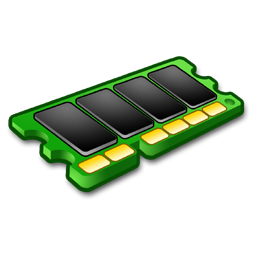
\includegraphics[width=.20\textwidth]{images/cpu-mem.png}};

    \node[inner sep=0pt, right=of cpu-mem] (gpu-mem)
    {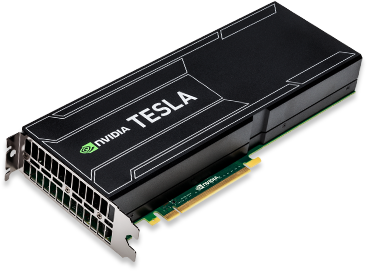
\includegraphics[width=.20\textwidth]{images/gpu-card.png}};

    \draw[*->] let \p1 = (block-5-2.one), \p2 = (block-5-2.center) in (\x1,\y2)    -- (CPU_device);
    \draw[*->] let \p1 = (block-5-2.second), \p2 = (block-5-2.center) in (\x1,\y2) -- (GPU_device);

    \draw[*->] (CPU_device-6-2.center) -- (cpu-mem);
    \draw[*->] (GPU_device-6-2.center) -- (gpu-mem);
  \end{tikzpicture}
  \caption{\texttt{Block} and \texttt{Device\_Info} structure}\label{fig:Device_Info_Structure}
\end{figure}

Using the meta data and specifically \texttt{data\_version\_}, the runtime can keep
track of changes in data on different devices and find the device with latest
data by comparing version numbers:

\begin{algorithm} {Block::get\_latest\_device() $\rightarrow$ Device\_Info}
  \singlespacing

  \begin{algorithmic}[1]
    \Function{Block::get\_latest\_device}{}
    \State $highest\_version\_found \gets 0$
    \State $highest\_version\_device \gets null$
    \ForAll{$device\_info\ in\ this.devices$}
    \If{$device\_info.data\_version > highest\_version\_found$}
    \State {$highest\_version\_found \gets info.data\_version$}
    \State {$highest\_version\_device \gets device\_info$}
    \EndIf
    \EndFor
    \State \Return $highest\_version\_device$
    \EndFunction
    % \hline
  \end{algorithmic}
\end{algorithm}

After determining the device with latest version of data, the runtime can update
other devices if needed. The only interfacing function exposed outside of
\texttt{Block} class is \texttt{get\_data(deviceid)} which returns pointer to memory
location on device identified by \texttt{deviceid}. The logic to always return
latest version of data can be embedded into \texttt{get\_data(device)}:

\begin{algorithm}  {Block::get\_data(deviceid) $\rightarrow$ double*}
  \singlespacing

  \begin{algorithmic}[1]
    \Function{Block::get\_data}{deviceid}
    \State $latest\_device \gets this.get\_latest\_device()$
    \If{$latest\_device.data\_version > this.devices[deviceid]$}
    \State {$memcpy(latest\_device.data,\ this.devices[deviceid].data)$}
    \EndIf
    \State \Return $this.devices[deviceid].data$
    \EndFunction
    % \hline
  \end{algorithmic}
  \label{alg:get_data}
\end{algorithm}

\section{Optimizing Block Copying}
A enormous cost has to be paid~\cite{Bakkum2010}\cite{memorytransferoverhead}
for transferring memory to GPU as compared to the time taken for actual computation
on GPU. Hence to have significant speed gains by executing on GPU over executing
on CPU, it is necessary to minimize time spent on block transfers. This has been
achieved in by deploying multiple optimizations that are explained in this section.

\subsection{Reducing Block Transfers}
The SIAL runtime has the information about intent of each block request, whether
the block is being requested to be read, updated or written. Using this information the
number of synchronizations between devices can be reduced. The blocks which are
going to be written need not be synchronized, however the blocks requested for
being read or updated need to be synchronized for the requested device.

The algorithm presented in~\ref{alg:get_data} can be split into
\texttt{get\_data} and a explicit \texttt{update\_data}:

\begin{algorithm}  {Block::get\_data(deviceid) $\rightarrow$ double*}
  \singlespacing

  \begin{algorithmic}[1]
    \Function{Block::get\_data}{deviceid}
    \State \Return $this.devices[deviceid].data$
    \EndFunction
    \\
    \Function{Block::update\_data}{deviceid}
    \State $latest\_device \gets this.get\_latest\_device()$
    \If{$latest\_device.data\_version > this.devices[deviceid]$}
    \State {$memcpy(latest\_device.data,\ this.devices[deviceid].data)$}
    \EndIf
    \EndFunction
    % \hline
  \end{algorithmic}
\end{algorithm}

This relatively simple change in organization of code along with the information
about intent of the request reduced the synchronizations by TODO\%.

\subsection{Memory Pinning}\label{memory_pinning}
The memory allocated on CPU or main memory is pageable by default. The GPU cannot
access data on such pageable host memory~\cite{datatransferoptimization}
\cite{programmingguidecuda}. For this reason when a memory copy operation is requested
from host to the GPU, the CUDA driver first allocates a temporary \textbf{page locked},
or \textit{pinned} memory on host (main memory) and copies the host memory to the
temporary pinned memory and then finally transfers the memory from pinned memory
to GPU device memory.
\begin{figure}[h] %place figure "here"
  \begin{tikzpicture}[
    container/.style={draw=gray, inner sep=5mm},
    typetag/.style={draw=black, anchor=west, inner sep=2mm, text width=3cm},
    title/.style={draw=none, color=gray, inner sep=0pt}]

    \node[title]   (gpu-title)     at (0, 5) {GPU};
    \node[typetag] (gpu-ram)       at (0, 4) {DRAM};
    \node[title]   (cpu-title)     at (0, 2) {CPU};
    \node[typetag] (pinned)        at (0, 1) {Temporary Pinned Memory};
    \node[typetag] (main-pageable) at (4, 1) {Pageable Memory};

    \node[container, fit=(gpu-title)(gpu-ram)]               {};
    \node[container, fit=(cpu-title)(main-pageable)(pinned)] {};

    \draw[draw=black, solid, line width=1mm, fill=black,
    preaction={-triangle 90, thin, draw, shorten >=-1mm}] (main-pageable) -- (pinned.east);
    \draw[draw=black, solid, line width=1mm, fill=black,
    preaction={-triangle 90, thin, draw, shorten >=-1mm}] (pinned)        -- (gpu-ram.south);
  \end{tikzpicture}
  \caption{\texttt{memcpy} w/o memory pinning}\label{fig:wo_mem_pin}
\end{figure}

Due to this copying of data to first a temporary page locked memory, extra time
is spent in redudant copy operation. To overcome this, the host memory can directly
be allocated in pinned memory. For this CUDA gives API \texttt{cudaMallocHost()},
\texttt{cudaHostAlloc()} to allocte memory and \texttt{cudaFreeHost()} to deallocate
the memory. Using this technique the data flow presented in~\ref{fig:wo_mem_pin} is
modified to flow presented in~\ref{fig:w_mem_pin}.
as:

\begin{figure}[h] %place figure "here"
  \begin{tikzpicture}[
    container/.style={draw=gray, inner sep=5mm},
    typetag/.style={draw=black, anchor=west, inner sep=2mm},
    title/.style={draw=none, color=gray, inner sep=0pt}]

    \node[title]   (gpu-title)     at (0, 5) {GPU};
    \node[typetag] (gpu-ram)       at (0.7, 4) {DRAM};
    \node[title]   (cpu-title)     at (0, 2) {CPU};
    \node[typetag] (pinned)        at (0, 1) {Pinned Memory};

    \node[container, fit=(gpu-title)(gpu-ram)] {};
    \node[container, fit=(cpu-title)(pinned)]  {};

    \draw[draw=black, solid, line width=1mm, fill=black,
    preaction={-triangle 90, thin, draw, shorten >=-1mm}] (pinned) -- (gpu-ram.south);
  \end{tikzpicture}
  \caption{\texttt{memcpy} with memory pinning}\label{fig:w_mem_pin}
\end{figure}

\subsubsection{Page Locked Memory Bandwidth}
Apart from saving a redudant copy operation, memory page locking also helps in
reducing time to copy because when memory is page locked, the GPU can invoke Direct
Memory Access (DMA)
controller~\cite{dmatransfer}\cite{whypinnedfast}\cite{teslaspecs}\cite{teslakspecs}
to transfer memory bypassing the CPU. This results in
twice~\cite{datatransferoptimization} the bandwidth between host and GPU.

\subsubsection{Asynchronous \texttt{memcpy}}
Since CUDA controller can invoke DMA controller to copy memory if the host memory
is page locked, this operation can be carried out asychronous not only to host but
also asychronously to GPU kernel execution engine. Thus both host and GPU can carry
on with execution of calculation while the blocks are synchronized. This is
elaborated in section~\ref{nonblockdevicesync}.

\subsubsection{Reusing Page Locked Memory Pages}
TODO.

\subsection{GPU Streams}
A \textit{stream} in CUDA is a sequence of operations that execute on the device
in the order in which they are issued by the host~\cite{overlapdatatransfer}.
Streams can be considered as operation pipes in which the operations get evaluated in
FIFO (First In First Out) fashion. Operations in different streams can be interleaved
and CUDA driver might execute them concurrently.

\subsubsection{Non Blocking Device Synchronization}\label{nonblockdevicesync}
GPU streams were used to implement non blocking SIA blocks synchronization. Using
multiple CUDA streams and page locked memory, DMA controllers can be invoked to
transfer memory from host to GPU and vice-versa asynchronously to both CPU and GPU
kernel execution engine. Current generation of GPU have dual DMA
controllers~\cite{teslaspecs}\cite{teslakspecs} and one kernel execution engine.
This means that the GPU can handle 2 asynchronous memory copying operation concurrently.
These hardware features have been exploited by implementing asynchronous memory
copying for block synchronization.

To implement the non blocking synchronization, multiple streams are created and
stored in the module \texttt{gpu\_super\_instructions} that initializes and
maintains the GPU state. The number of streams created is configurable and currently
is set to 2 since current generation of GPU devices have 2 DMA controllers. Each
\texttt{Device\_Info} object stores \texttt{gpu\_stream\_id} which is set when a
copy operation on \texttt{Block} object is initiated. At same time a bit
\texttt{isAsync} is set to denote that the \texttt{Block} object has pending
asynchronous operations. Before deferencing the memory pointer, runtime should
wait for the operation to finish by using CUDA call \texttt{cudaStreamSynchronize}.

\begin{algorithm} {Asynchronous Block Synchronization}
  \singlespacing

  \begin{algorithmic}[1]
    \Function{gpu\_memcpy}{src\_device, dest\_device, num\_elements}
    \State $next\_stream \gets get\_next\_stream()$
    \State $cudaMemcpyAsync(src\_device.data, dest\_device.data, num\_elements, next\_stream)$
    \State {$dest\_device.stream\_id \gets next\_stream$}
    \State {$dest\_device.isAsync \gets true$}
    \EndFunction
    \\
    \Function{block::get\_data}{deviceid}
    \If{$this.devices[deviceid].isAsync$}
    \State $cudaStreamSynchronize(this.devices[deiceid].stream\_id)$
    \State $this.devices[deviceid].isAsync \gets false$
    \EndIf
    \State \Return {$this.devices[deviceid].data$}
    \EndFunction
    % \hline
  \end{algorithmic}
\end{algorithm}

\section{GPU Buffers in Internode Communication}
SIAL makes it possible to work extremly large arrays by dividing the array into
multiple blocks and then server distributing the blocks to workers. Workers and
Server nodes communicate using highly optimized MPI library. Since GPU have their
own memory, using GPU for computation in a multinode environment can add an
additional layer of communication between GPU and network cards. In this section
optimizations for this communication are presented.

\subsection{Background}
GPU cards have their own memory on which the GPU can compute. In
Section~\ref{memory_pinning} the techniques used for optimizing memory transfer
between host memory (main memory) and GPU memory is discussed. Additionally when
MPI is used for internode communication, the data buffers to send are staged
to MPI buffers automatically by MPI. To send a buffer allocated on GPU using MPI,
it first has to be copied to main memory so that its pointer can be passed to
MPI functions like \texttt{MPI\_Send}/\texttt{MPI\_Recv}. Thus when GPU are used
along with MPI to send a unpinned memory buffer, in all there will 3 memory copy
operations and 6 in total if we consider memory operations on the destination node.
These operations are represented in Figure~\ref{fig:gpu_buff_transfer} by black arrows.

\subsection{MPI Transfers Using DMA}
After page locking a memory buffer, the CUDA driver and network fabric driver can
share it. Thus two set of copy operations can be saved by requesting page locked
buffers. This transfer is represented in Figure~\ref{fig:gpu_buff_transfer} by blue
arrows. It is worth noting that though this saves couple of copy operations, the
buffers still are managed through CPU memory and thus are limited by the CPU
memory bandwidth. SIA will make use of this when the buffers are page locked and
software libraries \& hardware facilities are not present for RDMA which is
presented next.

\subsection{MPI Transfers Using RDMA}
The intermediate copying operations to host memory can be avoided further by
taking advantage of Remote Direct Memory Access (RDMA). RDMA is a technique using
which the GPU can send buffers from GPU memory to network adapter without staging
through host memory. OpenMPI supports RDMA~\cite{openmpi-cudaaware} and thus all
the extra copy operations can be avoided.
Further RDMA transfers work independently of the CPU and thus it not only saves
extra copy operations, the transfer is done over PCI-E and is independent
of the CPU memory bandwidth and the memory bus traffic congestion.
This is conceptually represented in Figure~\ref{fig:gpu_buff_transfer} using orange
arrows which denotes one transfer from source GPU memory to destination GPU memory.
However, the servers in SIA are not allocated GPU since servers are not responsible
for any heavy calculation on blocks. They just manage blocks from workers and
swap \textit{inactive} blocks to disk. Hence a more accurate representation of
use of RDMA in SIA is presented in Figure~\ref{fig:gpu_buff_SIA}.

\begin{figure}[h] %place figure "here"
  \begin{tikzpicture}[
    container/.style={draw=gray, inner sep=5mm},
    typetag/.style={draw=black, anchor=west, inner sep=2mm, text width=1.5cm},
    title/.style={draw=none, color=gray, inner sep=0pt},
    thickarrow/.style={->, draw=black, thick, line width=1mm, shorten <= 2pt,
      shorten >= 2pt},
    thickblue/.style={<-, draw=blue, thick, line width=1mm, shorten <= 2pt,
      shorten >= 2pt, bend right=45},
    thickorange/.style={<-, draw=orange, thick, line width=1mm, shorten <= 2pt,
      shorten >= 2pt, bend right=10}]

    \node[title]   (gpu-title1)     at (0, 5) {SRC GPU};
    \node[typetag] (gpu-ram1)       at (0, 4) {DRAM};
    \node[title]   (cpu-title1)     at (0, 2) {SRC CPU};
    \node[typetag] (pinned1)        at (0, 1) {Pinned Memory};
    \node[typetag] (main-pageable1) at (2.5, 1) {Pageable Memory};
    \node[typetag] (mpi-buff1)      at (5, 1) {MPI Buffer}
      edge[thickblue] (pinned1);

    \node[title]   (gpu-title2)     at (14, 5) {DEST GPU};
    \node[typetag] (gpu-ram2)       at (14, 4) {DRAM}
      edge[thickorange] (gpu-ram1);
    \node[title]   (cpu-title2)     at (9, 2) {DEST CPU};
    \node[typetag] (mpi-buff2)      at (9, 1) {MPI Buffer};
    \node[typetag] (main-pageable2) at (11.5, 1) {Pageable Memory};
    \node[typetag] (pinned2)        at (14, 1) {Pinned Memory}
      edge[thickblue] (mpi-buff2);

    \node[container, fit=(gpu-title1)(gpu-ram1)]                           {};
    \node[container, fit=(cpu-title1)(main-pageable1)(pinned1)(mpi-buff1)] {};

    \node[container, fit=(gpu-title2)(gpu-ram2)]                           {};
    \node[container, fit=(cpu-title2)(main-pageable2)(pinned2)(mpi-buff2)] {};

    % Black arrows for src
    \draw[thickarrow] (gpu-ram1.south)      -- (pinned1.north);
    \draw[thickarrow] (pinned1.east)        -- (main-pageable1.west);
    \draw[thickarrow] (main-pageable1.east) -- (mpi-buff1.west);

    % Black arrow for network transfer
    \draw[thickarrow] (mpi-buff1.east)      -- (mpi-buff2.west);

    % Black arrows for dest
    \draw[thickarrow] (mpi-buff2.east)      -- (main-pageable2.west);
    \draw[thickarrow] (main-pageable2.east) -- (pinned2.west);
    \draw[thickarrow] (pinned2.north)       -- (gpu-ram2.south);

    % Legend
    \node[draw=none] (l-cuda-arrow) at (0, -1) {}
      edge[thickarrow, draw=orange] (1, -1);
    \node[draw=none, text=black, right=of l-cuda-arrow] {\footnotesize RDMA Transfers using CUDA-Aware MPI};
    \node[draw=none] (l-pinned-arrow) at (0, -1.5) {}
      edge[thickarrow, draw=blue]  (1, -1.5);
    \node[draw=none, text=black, right=of l-pinned-arrow] {\footnotesize DMA Transfers using Pinned Memory};
    \node[draw=none] (l-none-arrow) at (0, -2) {}
      edge[thickarrow]  (1, -2);
    \node[draw=none, text=black, right=of l-none-arrow] {\footnotesize Normal Transfer};
    %\draw[thickarrow] (pinned1.north)   to[out=90, in=90] (mpi-buff1.north);
    %\draw[thickarrow] (mpi-buff2.north) to[out=90, in=90] (pinned2.north);
  \end{tikzpicture}
  \caption{RDMA, DMA and normal transmission between two nodes with GPU}\label{fig:gpu_buff_transfer}
\end{figure}

\begin{figure}[h] %place figure "here"
  \begin{tikzpicture}[
    container/.style={draw=gray, inner sep=5mm},
    typetag/.style={draw=black, anchor=west, inner sep=2mm, text width=1.5cm},
    title/.style={draw=none, color=gray, inner sep=0pt},
    thickarrow/.style={->, draw=black, thick, line width=1mm, shorten <= 2pt,
      shorten >= 2pt},
    thickblue/.style={<-, draw=blue, thick, line width=1mm, shorten <= 2pt,
      shorten >= 2pt, bend right=45},
    thickorange/.style={<-, draw=orange, thick, line width=1mm, shorten <= 2pt,
      shorten >= 2pt, bend right=10}]

    \node[title]   (gpu-title1)     at (0, 5) {Worker GPU};
    \node[typetag] (gpu-ram1)       at (0, 4) {DRAM};
    \node[title]   (cpu-title1)     at (0, 2) {Worker CPU};
    \node[typetag] (pinned1)        at (0, 1) {Pinned Memory};
    \node[typetag] (main-pageable1) at (2.5, 1) {Pageable Memory};
    \node[typetag] (mpi-buff1)      at (5, 1) {MPI Buffer}
      edge[thickblue] (pinned1);

    \node[title]   (cpu-title2)     at (9, 2) {Server CPU};
    \node[typetag] (mpi-buff2)      at (9, 1) {MPI Buffer}
      edge[thickorange] (gpu-ram1);
    \node[typetag] (main-pageable2) at (11.5, 1) {Pageable Memory};

    \node[container, fit=(gpu-title1)(gpu-ram1)]                           {};
    \node[container, fit=(cpu-title1)(main-pageable1)(pinned1)(mpi-buff1)] {};

    \node[container, fit=(cpu-title2)(main-pageable2)(mpi-buff2)] {};

    % Black arrows for worker
    \draw[thickarrow] (gpu-ram1.south)      -- (pinned1.north);
    \draw[thickarrow] (pinned1.east)        -- (main-pageable1.west);
    \draw[thickarrow] (main-pageable1.east) -- (mpi-buff1.west);

    % Black arrow for network transfer
    \draw[thickarrow] (mpi-buff1.east)      -- (mpi-buff2.west);

    % Black arrows for dest
    \draw[thickarrow] (mpi-buff2.east)      -- (main-pageable2.west);

    % Legend
    \node[draw=none] (l-cuda-arrow) at (0, -1) {}
      edge[thickarrow, draw=orange] (1, -1);
    \node[draw=none, text=black, right=of l-cuda-arrow] {\footnotesize RDMA Transfers using CUDA-Aware MPI};
    \node[draw=none] (l-pinned-arrow) at (0, -1.5) {}
      edge[thickarrow, draw=blue]  (1, -1.5);
    \node[draw=none, text=black, right=of l-pinned-arrow] {\footnotesize DMA Transfers using Pinned Memory};
    \node[draw=none] (l-none-arrow) at (0, -2) {}
      edge[thickarrow]  (1, -2);
    \node[draw=none, text=black, right=of l-none-arrow] {\footnotesize Normal Transfer};
    %\draw[thickarrow] (pinned1.north)   to[out=90, in=90] (mpi-buff1.north);
    %\draw[thickarrow] (mpi-buff2.north) to[out=90, in=90] (pinned2.north);
  \end{tikzpicture}
  \caption{RDMA, DMA and normal transmission in SIA}\label{fig:gpu_buff_SIA}
\end{figure}